\documentclass[letter, 10pt]{article}
\usepackage[utf8]{inputenc}
\usepackage[spanish, es-tabla]{babel}
\usepackage{amsfonts}
\usepackage{amsmath}
\usepackage[dvips]{graphicx}
\usepackage{graphicx}
\usepackage{subfigure} % subfiguras
\DeclareGraphicsExtensions{.bmp,.png,.pdf,.jpg}
\usepackage{xcolor,listings}%color support for listings
\usepackage{epstopdf}
\usepackage{algpseudocode}
\usepackage{algorithm}
\usepackage{url}
\usepackage{caption}
\usepackage[justification=centering]{caption}
\usepackage{cite}
\usepackage[top=3cm,bottom=3cm,left=3.5cm,right=3.5cm,footskip=1.5cm,headheight=1.5cm,headsep=.5cm,textheight=3cm]{geometry}



\begin{document}



\title{Análisis Inteligente de Datos \\ \begin{Large}Tarea 3\end{Large}}
\author{Paulina Aguila - Felipe Flores}
\date{14 de julio de 2016}

\maketitle


\begin{figure}[ht]
\begin{center}

\includegraphics[width=0.2\textwidth]{Images/Isotipo-Negro.png}\\
\end{center}
\end{figure}
\vspace{2cm}

\section{Reducción de Dimensionalidad para Clasificación}

La reducción de dimensionalidad es un proceso que tiene mucha importancia dentro del análisis de datos, ya que ayuda a la visualización y la exploración de los datos, también reduce el costo computacional del procesamiento de los datos debido a que son menos dimensiones. Otro beneficio importante de la reducción de dimensionalidad, es que reduce significativamente el riesgo de \textit{overfitting} o sobre ajuste del modelo.\\

En esta primera sección, se trabajará con datos sobre sonidos fonéticos que debe ser identificados con vocales del inglés británico. Los datos se representan en un espacio de 10 características ($d=10$), en donde 528 registros corresponden a datos de entrenamiento y 462 son datos de prueba. Los autores reportan que el mejor desempeño corresponde a un 56\% de accuracy y se alcanza con un modelo de vecinos más cercanos y una red neuronal artificial de radio basal.\\

A través del lenguaje de programación Python, se cargan los datos de la fuente \cite{D1} y se llevan a un dataframe de entrenamiento con 528 registros y un dataframe de prueba con 462 registros.\\

Para cada conjunto de datos (entrenamiento y test), se deben normalizar los datos. Este es un paso muy importante, ya que permite ajustar la escala de las variables a la varianza de la unidad, lo que hace que los valores de datos que se encuentran ubicados en los extremos, no ejerzan un peso excesivo en la función objetivo.\\

Utilizando PCA (Análisis de Componentes Principales) se genera una representación en dos dimensiones para el dataset inicial (10 dimensiones). La Figura \ref{G1.1}, muestra la clasificación que realiza PCA.

\begin{figure}[h]
\begin{center}
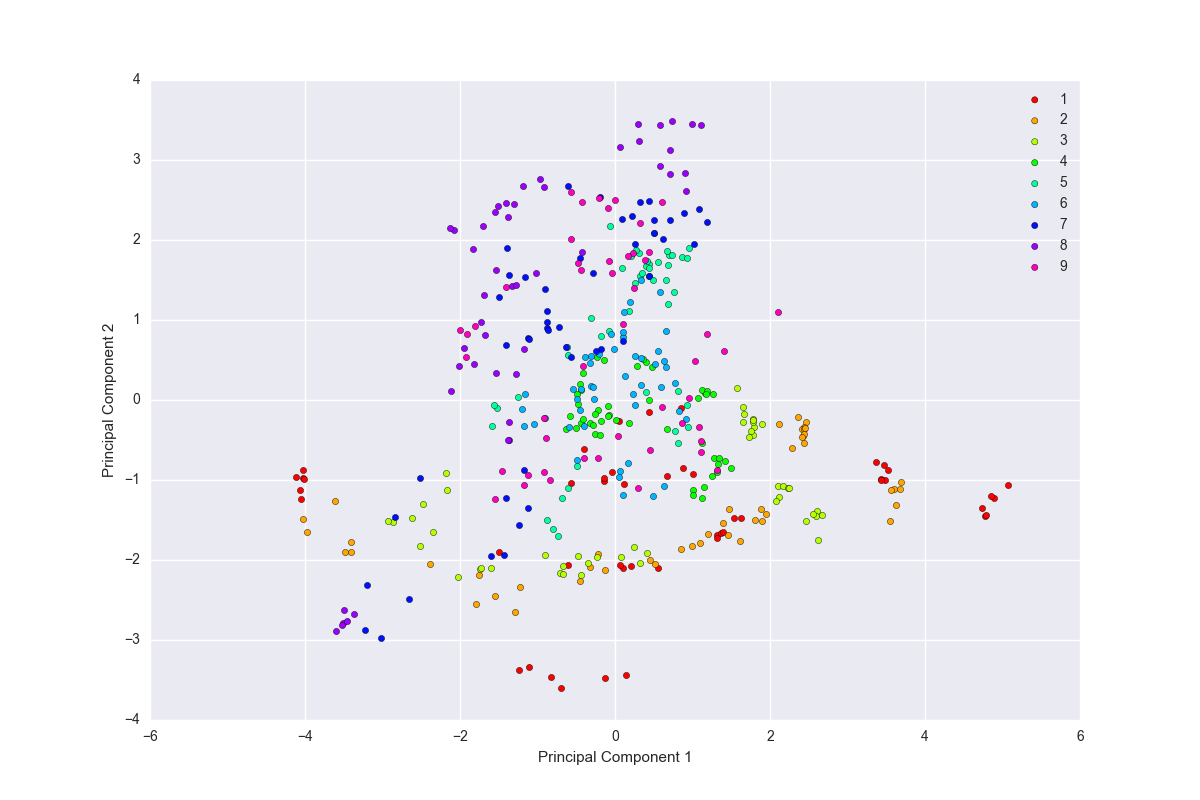
\includegraphics[width=1\textwidth]{Images/figure_1.png}
\caption{Gráfica que muestra las dos componentes principales de PCA diferenciando con distintos colores las 9 clases.}
\label{G1.1}
\end{center}
\end{figure}

Utilizando LDA (Linear Discriminant Analysis) se genera una representación en dos dimensiones para el dataset inicial (10 dimensiones). La Figura \ref{G1.2}, muestra la clasificación que realiza LDA.\\

\begin{figure}[h]
\begin{center}
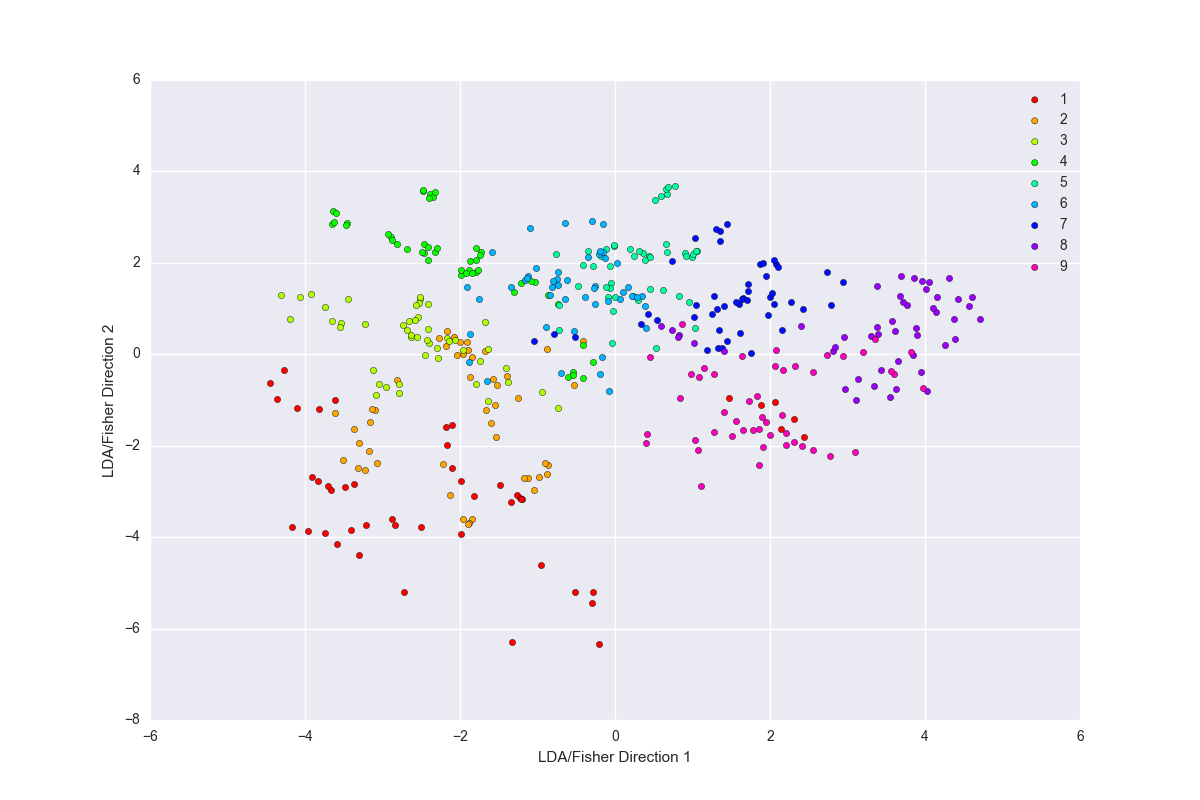
\includegraphics[width=1\textwidth]{Images/figure_2.png}
\caption{Gráfica que muestra las dos componentes principales de LDA diferenciando con distintos colores las 9 clases.}
\label{G1.2}
\end{center}
\end{figure}

Al analizar las Figuras \ref{G1.1} y \ref{G1.2}, se puede observar que en ambas se redujo la dimensionalidad de 10 a 2 componentes. Sin embargo, con PCA se observa que las clases no están separadas lo suficiente como para diferenciarlas, pero al utilizar LDA, se puede ver que las clases se separan más entre sí. Esto se puede deber a que LDA es un método de clasificación que en este caso se utiliza para reducir dimensionalidad y evitar el \textit{overfitting}.

\section{Análisis de Opiniones sobre Películas}

PIPE

\bibliographystyle{plain}
\bibliography{Referencias}

\end{document} 